\documentclass[a4paper]{easychair}

\usepackage{doc}
\usepackage{makeidx}

\usepackage{cite}
\usepackage{amssymb}
\usepackage{amsmath}
\usepackage{amsthm}
\usepackage{hyperref}
\usepackage{proof}
\usepackage{stmaryrd}
\usepackage{tikz}

\DeclareMathSizes{10}{9}{8}{7}

\bibliographystyle{plain}

%% Document
%%
\begin{document}\pagenumbering{gobble}

%% Front Matter
%%
\title{Closure Conversion for Dependent Type Theory, With Type-Passing Polymorphism\footnote{This work was supported by EFOP-3.6.3-VEKOP-16-2017-00002 grant.}}

\titlerunning{Closure Conversion for Dependent Type Theory, With Type-Passing Polymorphism}

\author{
  Andr{\'a}s Kov{\'a}cs
}

\institute{
  E{\"o}tv{\"o}s Lor{\'a}nd University, Budapest, Hungary \\
  \email{kovacsandras@inf.elte.hu}
}

\authorrunning{Kov{\'a}cs}

\clearpage

\maketitle

% this file is needed to build telescopes.tex

%% %% setting \sqcdot as HoTT-book-style transitivity
%% \makeatletter
%% \DeclareRobustCommand{\sqcdot}{\mathbin{\mathpalette\morphic@sqcdot\relax}}
%% \newcommand{\morphic@sqcdot}[2]{%
%%   \sbox\z@{$\m@th#1\centerdot$}%
%%   \ht\z@=.33333\ht\z@
%%   \vcenter{\box\z@}%
%% }
%% \makeatother


\renewcommand{\U}{\mathsf{U}}
\newcommand{\El}{\mathsf{El}}
\newcommand{\REN}{\mathsf{REN}}
\newcommand{\op}{\mathsf{op}}
\newcommand{\ra}{\rightarrow}
\newcommand{\Ra}{\Rightarrow}

\newcommand{\Set}{\mathsf{Set}}
\newcommand{\PSh}{\mathsf{PSh}}
\newcommand{\FamPSh}{\mathsf{FamPSh}}
\renewcommand{\ll}{\llbracket}
\providecommand{\rr}{\rrbracket}
\newcommand{\Con}{\mathsf{Con}}
\newcommand{\Ty}{\mathsf{Ty}}
\newcommand{\Tm}{\mathsf{Tm}}
\newcommand{\Tms}{\mathsf{Tms}}
\newcommand{\R}{\mathsf{R}}
\newcommand{\TM}{\mathsf{TM}}
\newcommand{\NE}{\mathsf{NE}}
\newcommand{\NF}{\mathsf{NF}}
\newcommand{\p}{\mathsf{p}}
\newcommand{\q}{\mathsf{q}}
\renewcommand{\u}{\mathsf{u}}
\renewcommand{\ne}{\mathsf{ne}}
\newcommand{\nf}{\mathsf{nf}}
\newcommand{\lQ}{\mathsf{lQ}}
\newcommand{\lU}{\mathsf{lU}}
\renewcommand{\lq}{\mathsf{lq}}
\newcommand{\lu}{\mathsf{lu}}
\newcommand{\cul}{\ulcorner}
\newcommand{\cur}{\urcorner}
\newcommand{\norm}{\mathsf{norm}}
\newcommand{\Nf}{\mathsf{Nf}}
\newcommand{\Ne}{\mathsf{Ne}}
\newcommand{\Nfs}{\mathsf{Nfs}}
\newcommand{\Nes}{\mathsf{Nes}}
\newcommand{\ID}{\mathsf{ID}}
\newcommand{\id}{\mathsf{id}}
\newcommand{\nat}{\,\dot{\rightarrow}\,}
%\newcommand{\nat}{\overset{\mathsf{n}}{\ra}} % this is how we denote it in the formalisation
\newcommand{\Nat}{\mathsf{Nat}}
\renewcommand{\S}{\overset{\mathsf{s}}{\ra}} % we have it with uppercase S in the formalisation
\newcommand{\blank}{\mathord{\hspace{1pt}\text{--}\hspace{1pt}}} %from the book
%\newcommand{\blank}{\!{-}\!}
\newcommand{\lam}{\mathsf{lam}}
\newcommand{\app}{\mathsf{app}}
\newcommand{\tr}[2]{\ensuremath{{}_{#1 *}\mathopen{}{#2}\mathclose{}}}
\renewcommand{\C}{\mathsf{C}}
\newcommand{\Code}{\mathsf{Code}}
\renewcommand{\M}{\mathsf{M}}
% from the book
%\newcommand{\M}{{\scalebox{0.6}{$\mathsf{M}$}}}
%% \newcommand{\C}{\mathcal{C}}
\newcommand{\data}{\mathsf{data}}
\newcommand{\ind}{\hspace{1em}}
\newcommand{\idP}{\mathsf{idP}}
\newcommand{\compP}{\mathsf{compP}}
\newcommand{\idF}{\mathsf{idF}}
\newcommand{\compF}{\mathsf{compF}}
\newcommand{\proj}{\mathsf{proj}}
\newcommand{\ExpPSh}{\mathsf{ExpPSh}}
\newcommand{\map}{\mathsf{map}}
\newcommand{\Var}{\mathsf{Var}}
\newcommand{\Vars}{\mathsf{Vars}}
\newcommand{\wk}{\mathsf{wk}}
\newcommand{\neuU}{\mathsf{neuU}}
\newcommand{\neuEl}{\mathsf{neuEl}}
\newcommand{\var}{\mathsf{var}}
\newcommand{\natn}{\mathsf{natn}}
\newcommand{\natS}{\mathsf{natS}}
\newcommand{\LET}{\mathsf{let}}
\newcommand{\IN}{\mathsf{in}}
\newcommand{\refl}{\mathsf{refl}}
\newcommand{\trans}{\mathbin{\raisebox{0.2ex}{$\displaystyle\centerdot$}}}
\newcommand{\zero}{\mathsf{zero}}
\newcommand{\suc}{\mathsf{suc}}
\newcommand{\N}{\mathbb{N}}

\newcommand\arcfrombottom{
  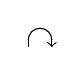
\begin{tikzpicture}[scale=0.03em]
    \draw (0,0) arc (0:180:0.5);
    \draw (0,0) edge[->] (0,-0.3);
    \draw (-1,0) edge (-1,-0.3);
  \end{tikzpicture}
}
\newcommand\arcfromtop{
  
\begin{tikzpicture}[scale=0.03em]
    \draw (0,0) arc (180:360:0.5);
    \draw (0,0) edge[->] (0,0.3);
    \draw (1,0) edge (1,0.3);
  \end{tikzpicture}
}

\newcommand{\Elim}{\mathsf{Elim}}
\newcommand{\elim}{\mathsf{elim}}
\newcommand{\Rec}{\mathsf{Rec}}
\newcommand{\record}{\mathsf{record}}
\newcommand{\funext}{\mathsf{funext}} \newcommand{\Q}{\mathsf{Q}}
\renewcommand{\T}{\mathsf{T}} \newcommand{\leaf}{\mathsf{leaf}}
\newcommand{\node}{\mathsf{node}} \newcommand{\perm}{\mathsf{perm}}
\newcommand{\coe}{\mathsf{coe}} \newcommand{\vz}{\mathsf{vz}}
\newcommand{\vs}{\mathsf{vs}} \newcommand{\untr}{\mathsf{untr}}
\newcommand{\from}{\mathsf{from}}
\newcommand{\fromeq}{{\mathsf{from}\hspace{-0.3em}\equiv}}
\newcommand{\fromsimeq}{{\mathsf{from}\hspace{-0.3em}\simeq}}
\newcommand{\Model}{\mathsf{Model}}
\newcommand{\DModel}{\mathsf{DModel}}
\newcommand{\module}{\mathsf{module}}
\newcommand{\open}{\mathsf{open}}
\renewcommand{\P}{\mathsf{P}} \newcommand{\Bool}{\mathsf{Bool}}
\newcommand{\true}{\mathsf{true}} \newcommand{\false}{\mathsf{false}}
\renewcommand{\not}{\mathsf{not}} \newcommand{\0}{\mathsf{0}}
\newcommand{\1}{\mathsf{1}} \renewcommand{\Pr}{\mathsf{Pr}}
\newcommand{\PrNat}{\mathsf{PrNat}} \newcommand{\J}{\mathsf{J}}
\newcommand{\wkV}{\mathsf{wkV}} \renewcommand{\r}[1]{{\P_{#1}}}
\newcommand{\stab}{\mathsf{stab}} \newcommand{\NTy}{\mathsf{NTy}}
\newcommand{\isDec}{\mathsf{isDec}} \newcommand{\dec}{\mathsf{dec}}
\newcommand{\yes}{\mathsf{yes}} \newcommand{\no}{\mathsf{no}}
\newcommand{\case}{\mathsf{case}} \newcommand{\inj}{\mathsf{inj}}
\newcommand{\K}{\mathsf{K}} \newcommand{\lb}{\langle}
\newcommand{\rb}{\rangle} \newcommand{\Decl}{\mathsf{Decl}}
\newcommand{\Core}{\mathsf{Core}} \newcommand{\IND}{\mathsf{ind}}
\newcommand{\Id}{\mathsf{Id}} \newcommand{\Base}{\mathsf{Base}}
\newcommand{\Setoid}{\mathsf{Setoid}}
\newcommand{\FamSetoid}{\mathsf{FamSetoid}}
\newcommand{\prop}{\mathsf{prop}} \newcommand{\resp}{\mathsf{resp}}
\newcommand{\transport}{\mathsf{transport}}
\newcommand{\I}{\mathsf{I}} \newcommand{\E}{\mathsf{E}}
\newcommand{\transp}{\mathsf{transp}}
\newcommand{\Transp}{\mathsf{Transp}}
\newcommand{\W}{\mathsf{W}}
\newcommand{\Fin}{\mathsf{Fin}} \newcommand{\fzero}{\mathsf{fzero}}
\newcommand{\fsuc}{\mathsf{fsuc}}
\newcommand{\inv}{\mathsf{inv}}
\newcommand{\con}{\mathsf{con}}
\newcommand{\LEFT}{\mathsf{left}}
\newcommand{\RIGHT}{\mathsf{right}}
\newcommand{\seg}{\mathsf{seg}}
\newcommand{\Int}{\mathsf{Int}}
\renewcommand{\in}{\mathbin{\hat:}}
%% \renewcommand{\hat}[1]{{\color{BrickRed}{#1}}}
\newcommand{\vdashh}{\mathbin{\hat\vdash}}
\newcommand{\rah}{\mathbin{\hat\ra}}
\newcommand{\commah}{\hat,\,}
\newcommand{\timesh}{\mathbin{\hat\times}}
\newcommand{\eqh}{\mathbin{\hat=}}
\newcommand{\TR}{\hat{\mathsf{tr}}}
\newcommand{\ap}{\hat{\mathsf{ap}}}
\newcommand{\apd}{\hat{\mathsf{apd}}}
\renewcommand{\tt}{\hat{\mathsf{tt}}}
\newcommand{\Tel}{\hat{\mathsf{Tel}}}
\newcommand{\Type}{\hat{\mathsf{Type}}}
\newcommand{\emptytel}{\hat{\epsilon}}
\newcommand{\telext}{\mathbin{\hat{\lhd}}}
\newcommand{\ltel}{\hat{\ll}}
\newcommand{\rtel}{\hat{\rr}}
\newcommand\pp{\ensuremath{\hat{\mathbin{+\mkern-10mu+}}}}
%% \newcommand{\semicol}{\hat;\,}
%% \newcommand{\targetass}{\hat{\Gamma}\semicol}
%\newcommand{\targetass}{;}


\pagestyle{empty}

%---------------------------------------------------------------------

Closure conversion is an early translation step in the compilation of
functional languages, which converts functions with potential free
variable occurrences to pairs consisting of environments and closed
functions. Environments carry values corresponding to free variables
of functions. The closed functions abstract over the captured
environments as well as the arguments of the original functions. This
representation allows an efficient environment-based execution model
where closed functions are compiled to shared immutable code segments.

Minamide et al. \cite{minamide1996typed} described type-preserving
closure conversion for a polymorphic language. They considered an
\emph{intensional} or \emph{type-passing} implementation of
polymorphism, which enables different memory layouts for differently
typed runtime objects, and necessitates that runtime type
representations are passed to polymorphic functions. In contrast,
\emph{type-erasing} polymorphism (as in \cite{morrisett1999system})
removes types during compilation, mandating uniform runtime
representations (although with potential layout-changing
optimizations, such as unboxing).

Generalizing type-passing polymorphism to dependent type theories
would allow precise specification of memory layout using dependent
types. For example, $\Sigma$-types may represent two values next to
each other in memory, where the size and layout of the second field
depends on the value of the first field. Hence, runtime objects would
be described by type-theoretic universes instead of simple statically
known layout schemes. Also, a closure-converted type theory with
precise control over memory layout could be useful as an intermediate
language even if types are erased somewhere on the way to machine
code.

The current work is a first step in this direction. I describe a
dependent type theory with a predicative universe hierarchy,
$\Sigma$-types, $\Pi$-types with \emph{closed} inhabitants and a novel
construction of closures. Consistency for this theory is proved with a
standard type-theoretic model. Then, it is proved that the general function
space with term formation in non-empty contexts is admissible in this
theory. General functions are represented as closures and term
formation corresponds to closure building. The expected $\beta$ and
$\eta$ rules also hold for this function space. Then, a closure
conversion translation into this theory is presented, from a source
theory with predicative universes and dependent
functions. Injectivity, preservation of typing and preservation of
conversion are proven for the translation.

\subsubsection*{Closures and type codes in the target theory}

The target theory has predicative universes $\U_i$ with decoding
$\El$, $\Sigma$-types, closed function types (denoted $(a : A)\ra B$)
and closure types $\Cl\,(a : A)\,B$. Closed functions differ from usual functions only
in the term formation rule: $\lambda$-abstraction is only valid in the
empty context (denoted $\boldsymbol{\cdot}$). For closures, there are
rules for type and term formation, elimination, and $\eta$ and $\beta$
conversion, presented in this order:

\begin{gathered}
  \infer{\Gamma \vdash \Cl\,(a : A)\,B\,\,\type_{\max(i,\,j)}}{\Gamma \vdash A\,\type_i & \Gamma, a : A \vdash B\,\type_j}
\hspace{2em}
  \infer{\Gamma \vdash \pack\,E\,env\,\,t : \Cl\,(a : A[e\mapsto env])\,(B[ea \mapsto (env,\,a)])}{\boldsymbol{\cdot} \vdash E : \U_i & \Gamma \vdash env : \El\, E & \boldsymbol{\cdot} \vdash t : (ea : \Sigma(e : \El\,E).A) \ra B}
\end{gathered}

\begin{gathered}
  \infer{\Gamma \vdash t\,u : B[a \mapsto u]}{\Gamma \vdash t : \Cl\,(a : A)\,B & \Gamma \vdash u : A}
  \hspace{1em}
  \infer{\Gamma \vdash t \equiv u}{\Gamma \vdash t : \Cl\,(a : A)\,B & \Gamma \vdash u : \Cl\,(a : A)\,B & \Gamma,\,a : A \vdash t\,a \equiv u\,a}
\end{gathered}
\vspace{-0.5em}
\begin{gather*}
  (\pack\,E\,env\,\,t)\,u \equiv t\,(env,\,u)
\end{gather*}

We use a primitive construction, in contrast to
\cite{minamide1996typed} where closures are derived from existential
types and translucent functions. The main reason is that universe
levels of captured environments can be arbitrarily high and need to be
hidden, which rules out $\Sigma$ representations. We can prove
consistency (and thus universe consistency) of $\Cl$ by a standard
type-theoretic model which unpacks environments and functions from
$\pack$, and applies the latter to the former, and elsewhere acts as
expected.

The type code inhabitants of $\U_i$ are themselves closure-converted:
for instance, a code for a $\Cl$ type contains a code for the domain
and a closure which computes the codomain type. This is because in a
type-passing implementation, type dependencies need to be computed at
runtime in a efficient manner. Decoding with $\El$ computes types from
codes by applying closures as needed. Rules for $\Cl$ codes are listed
below; cases for other types are analogous.
\vspace{0.5em}
\begin{gather*}
  \infer{\Gamma \vdash \mathsf{Cl'}\,A\,B : \U_{\max(i,\,j)}}
        {\Gamma \vdash A : \U_i & \Gamma \vdash B : \Cl\,(\El\,A)\,(\U_j)}
  \hspace{2.5em}
  \El\,(\mathsf{Cl'}\,A\,B)\equiv \Cl\,(a : \El\,A)\,(\El\,(B\,a))
\end{gather*}

\subsubsection*{Admissibility of general function space}

The main goal is to build a term of $\Cl\,(a : A)\,B$ from some $\Gamma, a : A \vdash t : B$, in a way such that $\beta$, $\eta$ and substitution rules hold. Closure building is defined mutually with quoting operations on well-formed contexts and types:

\begin{itemize}
\item From each $\Gamma$, we construct a closed code $\mathsf{quote}\,\,\Gamma$ for the corresponding iterated $\Sigma$-type, along with an isomorphism between $\Gamma$ and the singleton context containing $\El\,(\mathsf{quote}\,\,\Gamma)$, consisting of two back-and-forth substitutions.
\item From each $\Gamma \vdash A\,\,\type_i$, we construct $\Gamma \vdash \mathsf{quote}\,A : \U_i$, such that $\El$ retracts $\mathsf{quote}$, and $\mathsf{quote}$ is natural with respect to type substitution. Quoting to type codes here involves building closures which compute type dependencies, as we have seen for the $\Cl$ example.
\item Closures are built by $\pack$-ing together $\mathsf{quote}$-ed environment types, environments (given from $\Gamma$ \ra \El\,(\mathsf{quote}\,\,\Gamma)$ substitutions) and closed function bodies (given by closing the $t$ input function bodies using the $\El\,(\mathsf{quote}\,\,\Gamma) \ra \Gamma$ substitutions).
\end{itemize}

\subsubsection*{Closure conversion translation}

With admissible general function space at hand, closure conversion is given
by mutual induction on well-formed source syntax, converting source functions to closures.

\bibliography{b}

\end{document}
